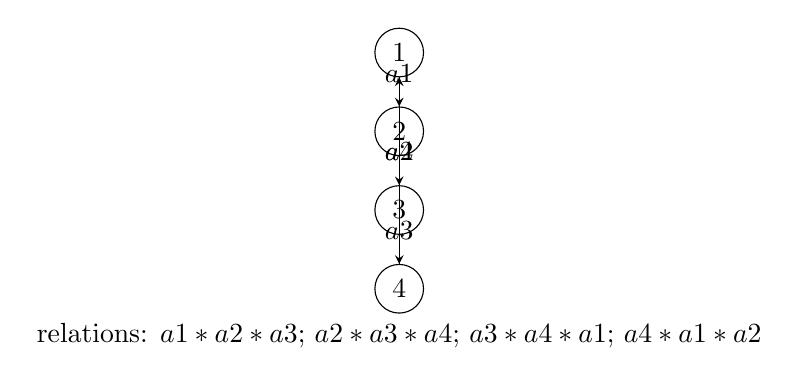
\begin{tikzpicture}[>=stealth]
  \node[draw, circle] (v1) at (0, {3/2}) {$1$};
  \node[draw, circle] (v2) at (0, {1/2}) {$2$};
  \node[draw, circle] (v3) at (0, {-1/2}) {$3$};
  \node[draw, circle] (v4) at (0, {-3/2}) {$4$};
  \draw[->] (v1) -- (v2) node[midway, above] {$a1$};
  \draw[->] (v2) -- (v3) node[midway, above] {$a2$};
  \draw[->] (v3) -- (v4) node[midway, above] {$a3$};
  \draw[->] (v4) -- (v1) node[midway, above] {$a4$};
  \node[align=left, below] at (current bounding box.south) {relations: $a1*a2*a3$;  $a2*a3*a4$;  $a3*a4*a1$;  $a4*a1*a2$};
\end{tikzpicture}
